%% LyX 2.4.0~RC3 created this file.  For more info, see https://www.lyx.org/.
%% Do not edit unless you really know what you are doing.
\documentclass[11pt,american]{article}
\usepackage[T1]{fontenc}
\usepackage[utf8]{inputenc}
\usepackage{geometry}
\geometry{verbose,tmargin=2cm,bmargin=2cm,lmargin=2cm,rmargin=2cm}
\usepackage{parskip}
\usepackage{babel}
\usepackage{amsmath}
\usepackage{amsthm}
\usepackage{graphicx}
\usepackage[pdfusetitle,
 bookmarks=true,bookmarksnumbered=false,bookmarksopen=false,
 breaklinks=false,pdfborder={0 0 0},pdfborderstyle={},backref=false,colorlinks=false]
 {hyperref}

\makeatletter
%%%%%%%%%%%%%%%%%%%%%%%%%%%%%% Textclass specific LaTeX commands.
\numberwithin{equation}{section}
\numberwithin{figure}{section}

\makeatother

\usepackage{listings}
\lstset{frame=lines,
breaklines=true,
breakatwhitespace=true,
basicstyle={\ttfamily \small}}
\renewcommand{\lstlistingname}{\inputencoding{latin9}Listing}

\begin{document}
\title{Solving Nonograms with ASP (working title)}
\author{Daniella Yordanova \and Fabian Kraus}
\maketitle
\begin{abstract}
...
\end{abstract}
\tableofcontents{}

\newpage{}

\section{Introduction to Nonograms}

...

test citation: \cite{NonogramRelaxationsPaper09}

\section{Solving Nonograms with ASP}

...

\subsection{Nonogram encoding}

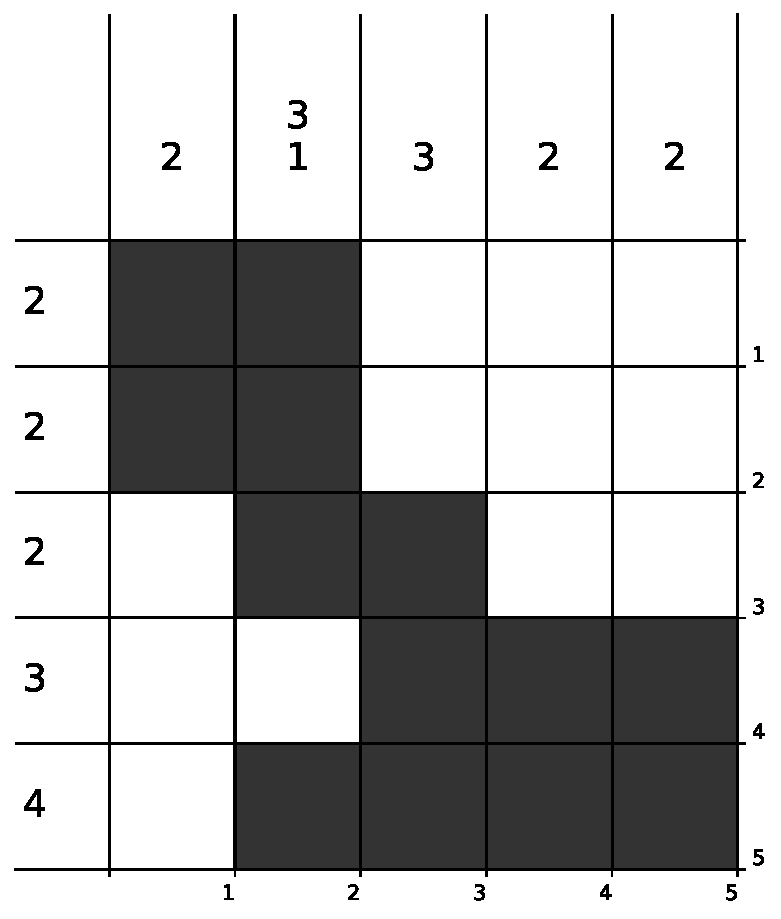
\includegraphics{example01}

We encode nonograms by adding a predicate corresponding to every line
and column hint. Shown below is an example of a 5x5 nonogram encoding:\lstinputlisting[language=Prolog,linerange={5-}]{../nonograms/example_01.lp}

Empty columns/rows can either be omitted entirely from the list, or
may have a single hint of length zero to indicate that no pixel in
this line is black.


\subsection{\emph{Brute Force} approach}

The first, most direct and least optimized attempt at a nonogram solver
using ASP will be referred to as the \emph{brute force} solver in
the following. It works like this: \\
First, define a rectangular pixel grid and indicate that every pixel
must have exactly one out of a given set of colors, in our case just
black (\bgroup\inputencoding{latin9}\lstinline!0!\egroup
) and white (\bgroup\inputencoding{latin9}\lstinline!1!\egroup
):\lstinputlisting[language=Prolog,linerange={9-14}]{../solvers/brute-force.lp}

Then impose the following three constraints independently for every
line (i.e. row or column) onto this black and white pixel grid:
\begin{enumerate}
\item The total number of black pixels must match the summed length of all
hints.
\item The first black pixel must be followed by exactly $l_{1}-1$ further
black pixels, where $l_{1}$ is the length of the first hint. The
$\left(l_{1}+1\right)$-th black pixel must be followed by exactly
$l_{2}-1$ further black pixels, where $l_{2}$ is the length of the
second hint, etc.
\item The pixel immediately after the $l_{1}$-th black pixel may not be
black. Similarly, the pixel immediately after the $\left(l_{1}+l_{2}\right)$-th
black pixel may not be black, etc.
\end{enumerate}
The first constraint can be implemented directly from the pixel grid:\lstinputlisting[language=Prolog,linerange={31-33}]{../solvers/brute-force.lp}

For formulating the other two constraints, a crucial piece of information
is the position of the first black pixel, the next first black pixel
after the first block, etc. For each hint, these positions are stored
using a helper predicate \bgroup\inputencoding{latin9}\lstinline!first_black\4!\egroup
, which is of the format \bgroup\inputencoding{latin9}\lstinline!first_black(line type, line number, block index, position)!\egroup
. Then constraints two and three may be encoded like this:\lstinputlisting[language=Prolog,linerange={53,54,57,58}]{../solvers/brute-force.lp}

Since all of these constraints are identical for rows and columns,
we added the following helper predicates used above for generalized
line handling:\lstinputlisting[language=Prolog,linerange={16-27}]{../solvers/brute-force.lp}This
has the advantage of only needing to formulate each constraint once,
instead of one variant for rows and one variant for columns.

\newpage{}

\bibliographystyle{plain}
\phantomsection\addcontentsline{toc}{section}{\refname}\bibliography{references}

\end{document}
